\section{Viola-Jones algoritam}

\subsection{Uvod}

Namena algoritma je detekcija i lokalizacija objekata na slici. Osmišljen od
strane Paul Viola i Michael Jones 2001. godine \cite{Viola2001RapidOD}.

Dugo godina je zbog brze i pouzdane detekcije bio standardan način detekcije
lica na slici. I danas je prisutan u velikom broju mobilnih telefona i
digitalnih kamera, ali danas postaje polako zamenjen konvolucionim neuronskim
mrežama. \\

Pouzdanost i brzina su postignuti uvođenjem tri ključna doprinosa:
\begin{itemize}

\item \textbf{Integralna slika} omogućava brzo izračunavanje obeležja.
\item \textbf{AdaBoost} algoritam za učenje, odabiranjem obeležja povećava
  brzinu i pouzdanost detekcije.
\item \textbf{Kaskadni klasifikator} Realizovanjem algoritma u kaskadama
  omogućava brzo odbacivanje pozadine slike kako je mala verovatnoća da će se tu
  naći lice. \\
\end{itemize}


\subsection{Integralna slika}

Kao jedan od ključnih delova algoritma, integralna slika omogućava izračunavanje
svakog pravougana obeležja u konstantnom vremenu.

Intenzitet piksela u integralnoj slici na poziciji x,y je zbir svih piksela koji
se nalaze gore i levo od pozicije x,y.

\begin{equation}
  \Scale[1.4]{ii(x,y)=\sum\limits_{x'\leq x, y'\leq y} i(x',y')}
  \label{IntegralImage_eq1}
\end{equation}

Gde je ii(x,y) integralna slika, a i(x,y) originalna slika. \\

\begin{figure}[h]
  \centering
  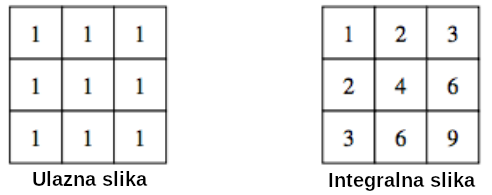
\includegraphics[width=8cm]{integral_image1}
  \caption{Primer integralne slike}
  \label{IntegralImage_img1}
\end{figure}

Piksele integralne slike je moguće računati u paraleli, ili
sekvencijalno. Izbor algoritma za računanje integralne slike značajno utiče na
performanse i potrebne hardverske resurse. \\
U paralelnoj implementaciji cena je
više pristupa memoriji i više potrebnih sabirača, dok je kod sekvencijalne
implementacije manja brzina. \\

Osobina koja integralnu sliku čini pogodnu za korišćenje u Viola-Jones algoritmu
je da je za računanje bilo koje pravougaone površine unutar integralne slike
potrebno 2 sabiranja i 2 oduzimanja.

\begin{figure}[h]
  \centering
  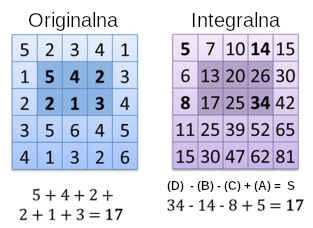
\includegraphics[width=8cm]{integral_image2}
  \caption{Primer računanja površine pravougaonika \cite{IntegralImage1_web}}
  \label{IntegralImage_img2}
\end{figure}

Na slici (\ref{IntegralImage_img2}) je prikazano računanje površine pravougaonika na
originalnoj slici i na integralnoj slici.
Kao što se može videti za površinu pravougaonika MxN na originalnoj slici nam je
potrebno MxN sabiranja. \\
Dok je kod integralne slike broj operacija 2 sabiranja i 2
oduzimanja i ne zavisi od dimenzija pravougaonika.

\begin{equation}
  \Scale[1.4]{\sum\limits_{(x,y)\in ABCD} i(x,y)=ii(D)+ii(A)-i(B)-ii(C)}
  \cite{Cen2016StudyOV}
  \label{IntegralImage_eq2}
\end{equation}